\documentclass{beamer}

\title{Terminal-based Motion-controlled Game Engine using OpenCV}
\author{A Clarke, Q Feng, J Spooner, L Squires}

\usecolortheme{whale}
\usepackage{graphicx}
\usepackage{calc}

\begin{document}
	
\frame{\titlepage}

\begin{frame}
	\frametitle{ARM Emulator and Assembler}
	Emulator:
	\begin{itemize}
		\item Load binary file into a \texttt{system\_state\_t} struct.
		\item Main loop:
		\begin{itemize}
			\item Execute the last decoded instruction, updating the \texttt{system\_state\_t} struct.
			\item Decode the last fetched instruction, producing an \texttt{instruction\_t} struct.
			\item Fetch the next instruction from memory, updating the PC.
		\end{itemize}
		\item Print the final system state.
	\end{itemize}
	Assembler:
	\begin{itemize}
		\item Load the assembly file.
		\item Tokenize instructions and generate symbol table.
		\item Create an \texttt{instruction\_t} struct representation of each instruction from tokens.
		\item Decode \texttt{instruction\_t} instructions into binary code.
		\item Write out binary file.
	\end{itemize}
\end{frame}

\begin{frame}
	\frametitle{ARM Emulator and Assembler (continued)}
	\begin{columns}
		\begin{column}{0.5\textwidth}
			\begin{itemize}
				\item Test script \texttt{src/run\_tests}
				\item Debug mode
				\item Raspberry Pi GPIO
			\end{itemize}
		\end{column}
		\begin{column}{0.5\textwidth}
			\begin{figure}
				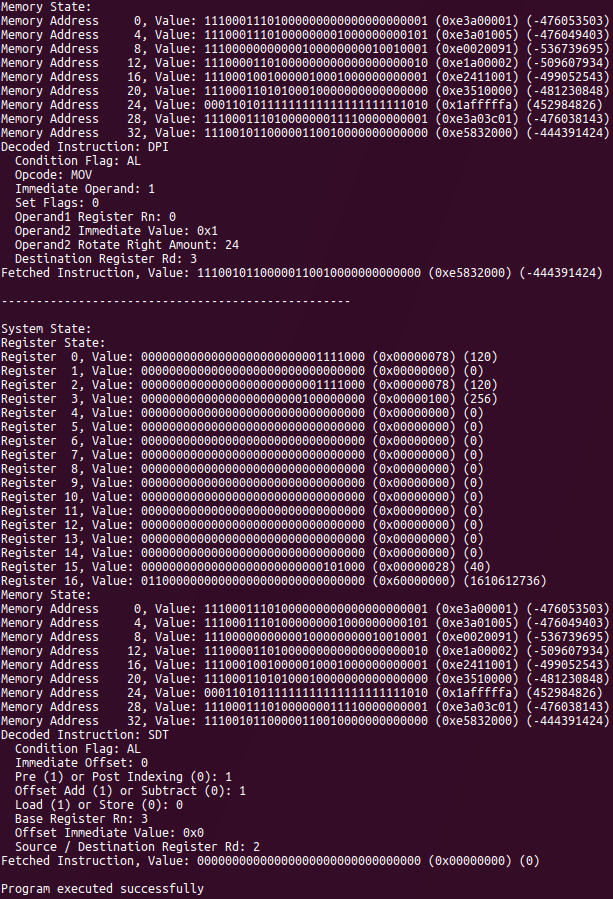
\includegraphics[width=\columnwidth-\columnsep]{Presentation/emulate.png}
			\end{figure}
		\end{column}
	\end{columns}
\end{frame}

\begin{frame}
	\frametitle{Overview of our Extension}
	\begin{itemize}
		\item Versatile ASCII game engine
		\item Arm tracking using OpenCV
		\item Getting started guide and full documentation
		\item Unit test suite
		\item Three example implementations (flappy bird, snake, pong)
	\end{itemize}
\end{frame}

\begin{frame}
	\frametitle{Terminal-based Game Engine}
	\begin{columns}
		\begin{column}{0.625\textwidth}
			\emph{Makes it easy to write terminal-based games}
			
			In the function template \texttt{init\_game}:
			\begin{enumerate}
				\item Define objects using \texttt{object\_list\_elem\_t}.
				\begin{enumerate}
					\item Type
					\item Position
					\item Velocity
					\item Acceleration
					\item ASCII representation (string, colour, size)
					\item Depth
					\item Pointer to another object
				\end{enumerate}
				\item Create collections of items (using \texttt{object\_list\_t}).
				\item Choose the \texttt{FRAMERATE}.
				\item Set up colour pairs.
			\end{enumerate}
		\end{column}
		\begin{column}{0.375\textwidth}
			\begin{figure}
				
\includegraphics[width=\columnwidth-\columnsep]{Presentation/snake.png}
			\end{figure}
		\end{column}
	\end{columns}
\end{frame}

\begin{frame}
	\frametitle{Terminal-based Game Engine (continued)}
	\begin{columns}
		\begin{column}{0.55\textwidth}
			\begin{figure}
				
\includegraphics[width=\columnwidth]{Presentation/flappy.png}
			\end{figure}
		\end{column}
		\begin{column}{0.45\textwidth}
			Write some simple helper functions to call on objects:
			\begin{enumerate}
				\setcounter{enumi}{3}
				\item E.g. \texttt{move}.
				\item E.g. \texttt{detect\_collision} (can use \texttt{is\_covering}).
			\end{enumerate}
			Complete the main game loop:
			\begin{enumerate}
				\setcounter{enumi}{5}
				\item Use \texttt{for\_all} to call \texttt{move} on objects.
				\item Call \texttt{print\_game}.
				\item Receive input using \texttt{getch}.
				\item Check game logic.
			\end{enumerate}
		\end{column}
	\end{columns}
\end{frame}

\begin{frame}
	\frametitle{Motion control using OpenCV}
	\begin{columns}
		\begin{column}{0.6\textwidth}
			\begin{itemize}
				\item Calibrate engine to users skin colour.
				\item Apply threshold to image using skin colour.
				\item Median blur to remove noise.
				\item Apply hand tracking algorithm.
			\end{itemize}
		\end{column}
		\begin{column}{0.4\textwidth}
			\begin{figure}
				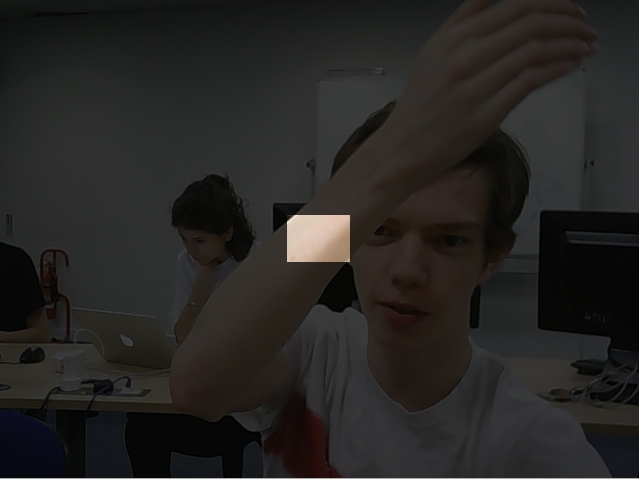
\includegraphics[width=\columnwidth-2\columnsep]{Presentation/calibration.png}
			\end{figure}
		\end{column}
	\end{columns}
	\begin{figure}
		
\includegraphics[width=\textwidth]{Presentation/opencv.png}
	\end{figure}
\end{frame}

\begin{frame}
	\frametitle{Motion control using OpenCV (continued)}
	\begin{itemize}
		\item Initialises to a guess position
		\item Updates each frame, moving towards high density regions
		\item If out of bounds, resets to guess
		\item Classifies based on position
	\end{itemize}
\end{frame}

\begin{frame}
	\frametitle{Demonstration}
	\texttt{setup\_engine}
	\begin{itemize}
		\item \texttt{open-cv-game-engine/flappy\_bird}
		\item \texttt{open-cv-game-engine/snake}
		\item \texttt{open-cv-game-engine/pong}
	\end{itemize}
\end{frame}

\begin{frame}
	\frametitle{Testing}
	\begin{itemize}
		\item Test script \texttt{open-cv-game-engine/run\_tests}
		\item Visual testing of motion control code
		\item Implementation of example games
	\end{itemize}
\end{frame}

\begin{frame}
\frametitle{Reflection}
\begin{itemize}
	\item Our group worked well together.
	\item We were always aware of what we should be doing, and what other members were doing.
\end{itemize}
\begin{figure}
	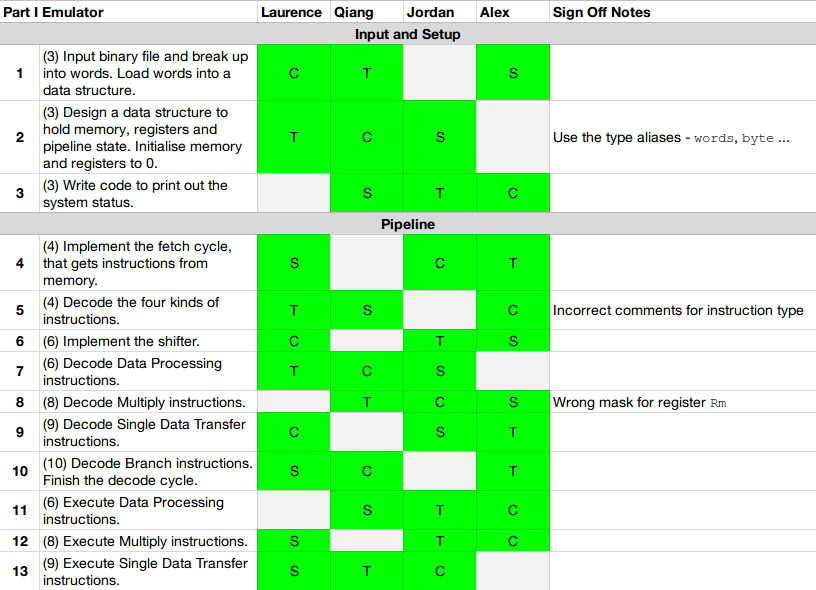
\includegraphics[width=0.7\textwidth]{Presentation/spreadsheet.png}
\end{figure}
\end{frame}

\begin{frame}
\frametitle{Reflection (continued)}
\begin{itemize}
	\item Split up the work well, so all members of the team contributing fairly equally.
	\item Could have researched and started our extension earlier.
	\item We would definitely keep our group's work ethic for the next project.
\end{itemize}
\end{frame}

\end{document}